\section{Frequency mode 22 and 24}
\label{sec:fm22}

\subsection{Overview}
\label{sec:fm22:overview}
Frequency modes~22 and 24 monitor the band around the \chem{CO} line at
$576.268\,\mathrm{GHz}$. Its main use is retrievals of \chem{CO} and when
possible \chem{O_3}. The receiver used for these modes suffered a failure
shortly after launch resulting in an inability to stabilise the frequency.
However it recovered between October 2003 until October 2004 for reasons that
can only be guessed at. In order to recover the \chem{CO} product a special
algorithm had to be developed to first detect if the \chem{CO} line was at
all present in the spectra of a given scan. This involved distinguishing the
\chem{CO} and \chem{O_3} lines and then if the \chem{CO} line was present
re-tuning the frequency scale. It was also necessary to account for rapid
changes in the frequency during a vertical scan and within the integration
time. The details are given in \cite{grieco2020a}.

Spectra from this observation mode are shown in Figure~\ref{fig:spectra:22}.

\begin{figure}[ht]
    \centering
    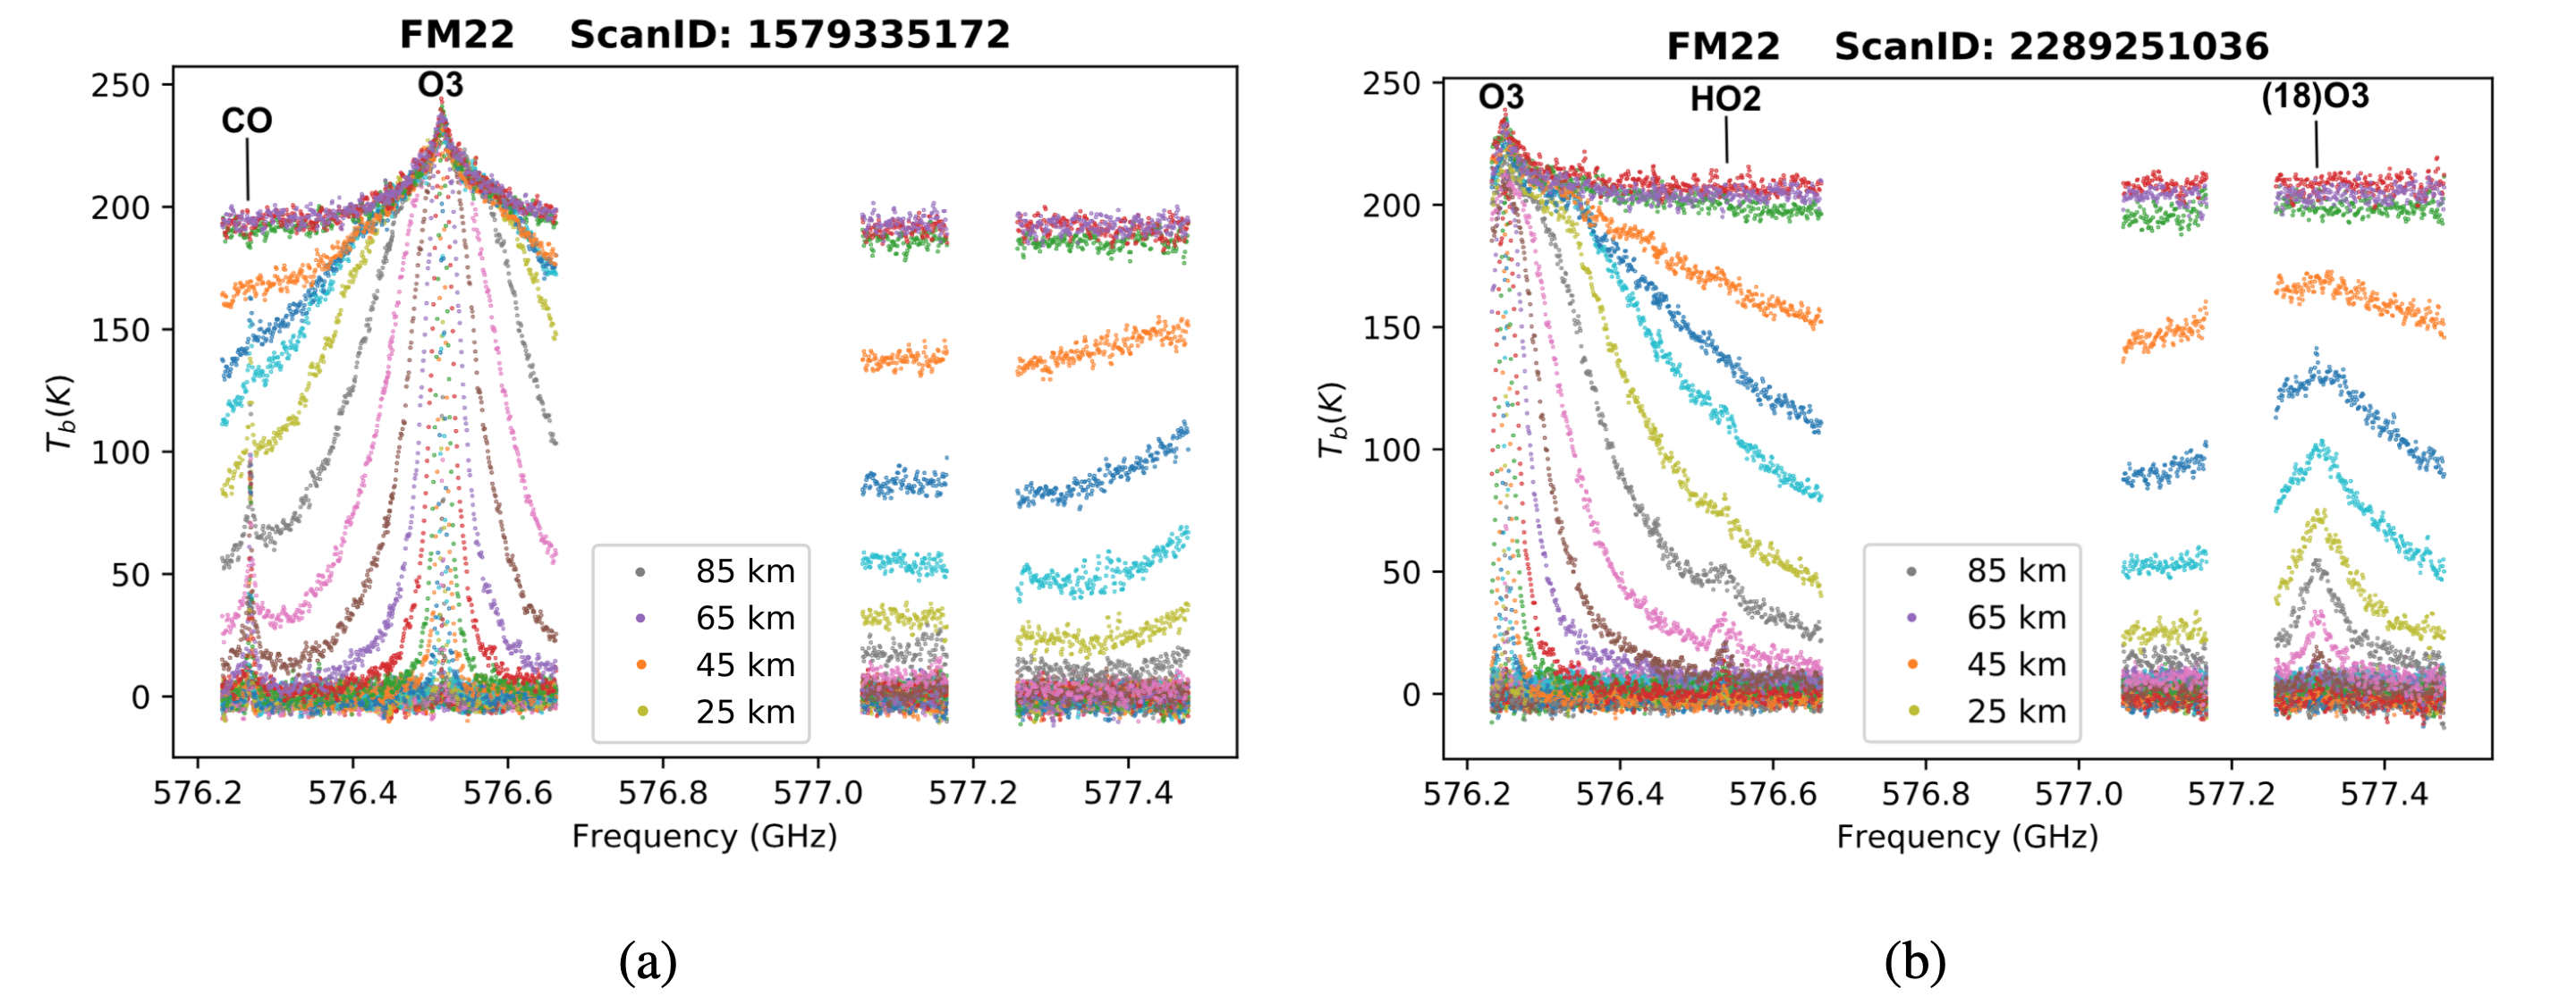
\includegraphics[width=0.95\textwidth]{../figures/spectra/fm_22}
    \caption{Spectra for the CO mode showing one example where the line is present and one without.
    }\label{fig:spectra:22}
\end{figure}


\subsection{Comparison of retrieved profiles}
\label{sec:fm22:comparison}


%%%%%%%
% CO %
%%%%%%%

\subsubsection{\chem{CO}}
\label{sec:fm22:comparison:CO}
The retrievals for \chem{CO} have been compared with data from the MIPAS and
MLS instruments.  The comparison does not follow the same methodology as for the other modes, rather a special approach has had to be employed. 
The  MIPAS instrument was operated in several modes and the most useful ones covering the extended altitude range of the Odin measurements are the Middle Atmosphere and the Upper atmosphere modes.  A detailed analysis in presented in \cite{grieco2020a} with only the conclusions presented here.

\subsection{Discussion}
\label{sec:fm22:discussion}
Comparisons with MIPAS, ACE-FTS and OSO show a positive bias of SMR of up to
+20~\% at low altitudes (50--60~km) and a negative bias of up to -20~\% at
high altitudes (80--115~km). Something different is found with regards to MLS
-- i.e. negative difference at all altitudes, ranging from -40~\% to -10~\%
-- which is in accordance with the stated MLS bias \cite{Errera2019}.



\subsection{Conclusions}
\label{sec:fm22:conclusions}
Based on the discussion above, the \chem(CO) data set has been recovered for a large fraction of the mission and can be used in the altitude range 50--115~km.
